\documentclass[17pt]{beamer} %Makes presentation
%\documentclass[handout, 17pt]{beamer} %Makes Handouts
\documentclass[14pt]{beamer} %Makes presentation
%\documentclass[handout]{beamer} %Makes Handouts
\usetheme{Singapore} %Gray with fade at top
\useoutertheme[subsection=false]{miniframes} %Supppress subsection in header
\useinnertheme{rectangles} %Itemize/Enumerate boxes
\usecolortheme{seagull} %Color theme
\usecolortheme{rose} %Inner color theme

\definecolor{light-gray}{gray}{0.75}
\definecolor{dark-gray}{gray}{0.55}
\setbeamercolor{item}{fg=light-gray}
\setbeamercolor{enumerate item}{fg=dark-gray}

\setbeamertemplate{navigation symbols}{}
%\setbeamertemplate{mini frames}[default]
\setbeamercovered{dynamics}
\setbeamerfont*{title}{size=\Large,series=\bfseries}

%\setbeameroption{notes on second screen} %Dual-Screen Notes
%\setbeameroption{show only notes} %Notes Output

\setbeamertemplate{frametitle}{\vspace{.5em}\bfseries\insertframetitle}
\newcommand{\heading}[1]{\noindent \textbf{#1}\\ \vspace{1em}}

\usepackage{bbding,color,multirow,times,ccaption,tabularx,graphicx,verbatim,booktabs,fixltx2e}
\usepackage{colortbl} %Table overlays
\usepackage[english]{babel}
\usepackage[latin1]{inputenc}
\usepackage[T1]{fontenc}
\usepackage{lmodern}

%\author[]{Thomas J. Leeper}
\institute[]{
  \inst{}%
  Department of Government\\London School of Economics and Political Science
}

\usepackage{tikz}
\usetikzlibrary{shapes,arrows,decorations.pathreplacing}
\usepackage[normalem]{ulem}
\setbeamertemplate{mini frames}{}

\title{Interviewing, Structured and Unstructured}

\date[]{}

\begin{document}

\frame{\titlepage}

\frame{\tableofcontents}


\frame{}

\section{Participant Observation}
\frame{\tableofcontents}
\frame{\tableofcontents[currentsection]}

\frame{
\frametitle{``Field work''}
\begin{itemize}\itemsep0.5em
\item Any research activity outside the university setting % soaking and poking
	\begin{itemize}\footnotesize
	\item Textual or archival searches
	\item Interviews (structured or unstructured)
	\item Focus groups
	\item Participant observation
	\item Some mix of these
	\end{itemize}
\item Term is agnostic about approach, theory, and method
\item Might be one-off, sporadic, or long-term
\end{itemize}
}

% continuum between observing processes directly and gathering secondary source evidence about processes that cannot be directly observed

\frame{
\frametitle{{\large Participant Observation}}

\small

\begin{itemize}
\item Definition: ``Participant observation is a research strategy whereby the researcher becomes involved in a social situation for the purpose of understanding the behaviour of those engaged in the setting\dots The outcome of the research is a detailed account of the activities and behaviour of those involved.''\footnote{p.265 from Burnham et al. 2008. \textit{Research Methods in Politics}. 2nd Edition. Palgrave.}
\end{itemize}
}


\frame{
\frametitle{{\large Participant Observation}}

\begin{itemize}\itemsep0.5em
\item<2-> Intentionally subjective/reflective; no belief in possible observational objectivity
\item<3-> Generally inductive in nature
\item<4-> Typically does not generate DSOs
\end{itemize}
}

% A common approach in case study research
% Breakdown of objectivity is this desirable or not?



\frame{
\frametitle{Assorted Examples}

\small

\begin{enumerate}
\item Goffman, A. 2014. \textit{On the Run: Fugitive Life in an American City}. Chicago.
\item<2-> Fenno, R. 1978. \textit{Home Style: U.S. House Members in their Districts}. Pearson.
\item<3-> Cramer, K. 2016. \textit{The Politics of Resentment}. Chicago.
\item<4-> Nielsen, R.K. 2012. \textit{Ground Wars}. Princeton.
\item<5-> Festinger, Riecken, and Schachter. 1956. \textit{When Prophecy Fails}. Harper.
\end{enumerate}

}





\frame{

\frametitle{Four Ideal Types\footnote{Gold, R. 1958. ``Roles in Sociological Field Observation.'' \textit{Social Forces} 36(3): 217--23.}}

\begin{enumerate}\itemsep1em
\item Complete participant
\item Participant as observer
\item Observer as participant
\item Complete observer
\end{enumerate}

}

\frame{
\frametitle{Complete participant}
\begin{itemize}\itemsep1em
\item Participate without disclosing observer/researcher role
\item Essentially covert (``being undercover'')
\item May be useful in sensitive domains
\item Raises ethical concerns
\end{itemize}
}

\frame{
\frametitle{Participant as observer}
\begin{itemize}\itemsep1em
\item Participate, but not fully
\item Retain explicit observer role
\item Negotiate exact role in the situation and access to group members and information
\end{itemize}
}

\frame{
\frametitle{Observer as participant}
\begin{itemize}\itemsep1em
\item Essentially interviews
\item Limited time frames
\item Note: Sometimes seen as indistinguishable from ``complete observer''
\end{itemize}
}

\frame{
\frametitle{Complete observer}
\begin{itemize}\itemsep1em
\item Purely observer role; no participation
\item Still requires negotiated access in many cases, but may not require the same types of consent as participant roles
\item Easier to keep a distance and avoid ``rapport'' with group members
\end{itemize}
}


\frame{
\frametitle{Participant vs. Observer}

\small

\begin{itemize}\itemsep0.25em
\item Not always a choice
	\begin{itemize}\footnotesize
	\item Access might be limited
	\item Ethical obligations
	\end{itemize}
\item<2-> Is situation public vs. private?
\item<3-> How does your presence change the situation?
\item<4-> How does being a participant change your interpretations of events?
\item<5-> How does being an observer change your interpretation of events?
\end{itemize}
}

% Where is Fenno on the continuum between participant and observer?
% Where is Goffman?


\frame{
\frametitle{{\large Ethnography vs. Journalism}}

\begin{center}
\Large What's the difference?
\end{center}

}

\frame{
\frametitle{Focus Groups}

\small

\begin{itemize}
\item Definition: ``A discussion among a small number of members of a target population, guided by a moderator.''\footnote{Groves et al. 2009. \textit{Survey Methodology}. 2nd Edition. Wiley.}
\item A descriptive bridge between interviewing and ethnography
	\begin{itemize}
	\item Less structured than an interview
	\item More structured than participant observation
	\item Typically brief (1-2 hours)
	\end{itemize}

% have any of you ever been in a focus group?
\end{itemize}
}

\frame{}

\section[Questionnaires]{Questionnaire Methods}
\frame{\tableofcontents[currentsection]}


\frame{

\frametitle{}


\begin{center}
In lieu of direct observation/participation, we may ask \textit{other people} to \textit{describe} the phenomena we are interested in by asking them \textit{questions}.
\end{center}

\small
\begin{itemize}
\item<2-> May generate DSOs
\item<3-> May generate other kinds of descriptions
\end{itemize}

}

\frame{
	\frametitle{Topics of questions}
	\begin{itemize}\itemsep1em
		\item Recall
			\begin{itemize}
    \item Behaviour
    \item Knowledge and beliefs
    \item Perceptions
    \item Demographics
			\end{itemize}
		\item Evaluation
			\begin{itemize}
			\item Opinions
			\end{itemize}
	\end{itemize}
}

\frame{
	\frametitle{Structure of a question}
	\begin{enumerate}\itemsep0.5em
		\item<2-> Survey mode
		\item<3-> Survey context
		\item<4-> Vignette or introductory text
		\item<5-> Question itself
		\item<6-> Response format and options
		\item<7-> Follow-ups, branches, checks, validation, clarification
	\end{enumerate}
}

\frame{
	\frametitle{{\large Questions as Operationalization}}
	
	\small
	\begin{itemize}\itemsep0.5em
		\item Questionnaires start with concept definition
		\item Multiple ways to operationalize any concept
		\item Important concepts may require multiple measures
		\item Question should measure concept of interest
	\end{itemize}
}

%\frame{\frametitle{How do we know if a survey response is ``true''?}}


%\frame{
%	\frametitle{Validation studies}
%	\begin{enumerate}\itemsep1em
%		\item Some survey responses can be \textit{validated}
%		\item Easy for some behavioural constructs
%		\item Direct observation, administrative data, etc.
%	\end{enumerate}
%}

\frame{
	\frametitle{Problem Set 4}
	
	\small
	\begin{itemize}\itemsep0.5em
	\item Work as class groups to conduct a ``pilot'' study
	\item Use a Eurobarometer survey of your choice
	\item Conduct in-person interviews
	\item Evaluate process of collecting interview data
	\end{itemize}
}

\frame{

\vspace{-1em}
\frametitle{{\normalsize Evaluating a questionnaire}}

\small

\begin{itemize}\itemsep-0.25em
	\item<2-> Is the question easy for respondents to understand?
	\item<3-> Are the number and types of response options appropriate?
	\item<4-> Are the categories sufficiently distinct from one another?
	\item<5-> Is a ``no opinion,'' ``don't know,'' or ``neither support nor oppose'' response option available?
	\item<6-> Is one survey item (i.e., one question) sufficient to measure this construct?
	\item<7-> How long does it take to read and answer this question?
\end{itemize}
}


\frame{}

\frame{

\vspace{-1em}
\frametitle{{\normalsize Cognitive interviewing methods}}

\begin{itemize}\itemsep0.75em
\item<2-> Retrospective think-alouds % (in which respondents describe how they arrive at their answers either just after they provide them or at the end of the interview)
\item<3-> Paraphrasing %(in which respondents restate the question in their own words)
\item<4-> Definitions %(in which respondents provide definitions for the key terms in the question)
\item<5-> Probes %(in which respondents answer follow-up questions designed to reveal their response strategies)
\item<6-> General discussion/evaluation
\end{itemize}

}

\subsection{Recall-type Questions}
%\frame{\tableofcontents[currentsubsection]}

\frame[label=recallquestions]{
	\frametitle{Recall-type Questions}
	\begin{itemize}\itemsep1em
		\item Knowledge
		\item Behaviour
		\item Events
	\end{itemize}
}


\frame{
	\frametitle{Recalling Knowledge}
	\begin{itemize}\itemsep1em
		\item Factual items with ``true'' responses
		    \begin{itemize}
		        \item Political knowledge
		        \item Knowledge about products/services
		        \item General knowledge
		    \end{itemize}
		\item How do we deal with ``don't know'' responses?
		    \begin{itemize}
		        \item Genuine expression of lack of knowledge?
		        \item Insufficient time to think?
		        \item Question was unclear/ambiguous?
		    \end{itemize}
	\end{itemize}
}

\frame{
	\frametitle{Recalling Behaviours}
	\begin{itemize}\itemsep1em
		\item Things respondent did in the past
            \begin{itemize}
                \item Media use
                \item Eating/dietary habits
                \item Past voting
            \end{itemize}
        \item Challenging to measure accurately
        \item Can (sometimes) be easily validated
	\end{itemize}
}

\frame{
	\frametitle{{\normalsize What affects responses to recall questions?}}
	
	\small
	
	\begin{itemize}\itemsep-0.25em
        \item Question misunderstanding
            \begin{itemize}
                \item Vague concepts
                \item Confusing or long wording
            \end{itemize}
        \item<2-> Forgetting
        \item<3-> Recency/primacy biases among responses
        \item<4-> Motivated misreporting
        \item<5-> Reference period ambiguity
        \item<6-> Rare events
        \item<7-> True ``don't know'' responses
	\end{itemize}
}


\frame{
	\frametitle{Motivated misreporting}
	\begin{itemize}\itemsep1em
        \item Intentionally giving an incorrect response
            \begin{itemize}
                \item Applies to recall and evaluative questions
            \end{itemize}
        \item<2-> Several common biases
            \begin{itemize}
                \item<3-> Social desirability bias
                \item<3-> Acquiescence bias
                \item<3-> Demand characteristics
            \end{itemize}
	\end{itemize}
}


\frame{}

\subsection{Evaluative Questions}
%\frame{\tableofcontents[currentsubsection]}

\frame{
	\frametitle{Evaluative questions}
	\begin{itemize}\itemsep1em
		\item Name an object of evaluation
		\item Possibly describe that object
		\item Ask for a transformation of the evaluation onto a set of responses
	\end{itemize}
}

\frame{
	\frametitle{Question templates}

	\small
	
	\begin{itemize}
		\item Ratings
			\begin{itemize}
				\item Several varieties of rating scales
			\end{itemize}
		\item Scales/Thermometers
		\item Agree-disagree
		\item Forced choices
		\item Open-ended
		\item Rankings (note: need alternatives to rank against)
	\end{itemize}
}

\frame{
	\frametitle{Additional Considerations}
	\begin{itemize}\itemsep0.5em
		\item How many response categories?
		\item Middle category (presence and label)
		\item ``no opinion'' and/or ``don't know'' options
		\item Probe if ``no opinion'' or ``don't know''?
		    \begin{itemize}
                \item Encourage guessing?
    		    \item Clarify/describe object of evaluation?
		    \end{itemize}
		\item Branching format?
		\item Order of response categories
		\item Changes based on survey mode
	\end{itemize}
}


\frame{
	\frametitle{Activity Example}
	\begin{itemize}\itemsep1em
		\item Public opinion survey in Great Britain
		\item Construct: Opinion toward UK involvement in air strikes on Islamic State militants in Iraq and Syria
		\item Think about strengths and weaknesses of each question
	\end{itemize}
}

\frame{
	\frametitle{{\large Example: Rating (bipolar)}}
	Do you support or oppose Great Britain's participation in U.S.-led air strikes on Islamic State (IS) in Iraq and Syria?
	\begin{itemize}
		\item Strongly support
		\item Somewhat support
		\item Neither support nor oppose
		\item Somewhat oppose
		\item Strongly oppose
	\end{itemize}
}

\frame{
	\frametitle{{\large Example: Rating (branching)}}
	
	\footnotesize
	
	Do you support or oppose Great Britain's participation in U.S.-led air strikes on Islamic State (IS) in Iraq and Syria?
	\begin{itemize}
		\item Support
		\item Neither support nor oppose
		\item Oppose
	\end{itemize}
	\vspace{1em}
	\only<2->{
	Would you say that you strongly [support|oppose] or somewhat [support|oppose] Great Britain's participation?
	\begin{itemize}
		\item Strongly
		\item Somewhat
	\end{itemize}
	}
}

\frame{
	\frametitle{{\large Example: Rating (bipolar)}}

	\small
	
	Are you favourable or unfavourable toward Great Britain's participation in U.S.-led air strikes on Islamic State (IS) in Iraq and Syria?
	\begin{itemize}
		\item Very favourable
		\item Somewhat favourable
		\item Neither favourable nor unfavourable
		\item Somewhat unfavourable
		\item Strongly unfavourable
	\end{itemize}
}

\frame{
	\frametitle{{\large Example: Rating (unipolar)}}
	To what extent do you support Great Britain's participation in U.S.-led air strikes on Islamic State (IS) in Iraq and Syria?
	\begin{itemize}
		\item Strongly
		\item Moderately
		\item Somewhat
		\item Not at all
	\end{itemize}
}

\frame{
	\frametitle{{\large Example: Rating (unipolar)}}
	How favourable are you toward Great Britain's participation in U.S.-led air strikes on Islamic State (IS) in Iraq and Syria?
	\begin{itemize}
		\item Extremely favourable
		\item Very favourable
		\item Moderately favourable
		\item Somewhat favourable
		\item Not at all favourable
	\end{itemize}
}

\frame{
	\frametitle{{\large Example: Numbered Scale}}
	
	\small
	
	On a scale from 1 to 5, with 1 being ``strongly oppose'' and 5 being ``strongly support,'' to what extent do you support Great Britain's participation in U.S.-led air strikes on Islamic State (IS) in Iraq and Syria?
	
	\footnotesize
	\begin{enumerate}
		\item Strongly oppose
		\item 
		\item 
		\item 
		\item Strongly support
	\end{enumerate}
}

\begin{frame}[fragile]
	\frametitle{{\large Example: Thermometer}}
	
	\footnotesize
	
	We would like to get your feelings toward some of political policies. Please rate your support for the policy using something we call the feeling thermometer. Ratings between 50 degrees and 100 degrees mean that you feel favourable and warm toward the policy. Ratings between 0 degrees and 50 degrees mean that you don't feel favourable toward the policy. You would rate the policy at the 50 degree mark if you don't feel particularly favourable or unfavourable toward.
	
	\vspace{1em}
	Great Britain's participation in U.S.-led air strikes on Islamic State (IS) in Iraq and Syria.
	
	\begin{center}
	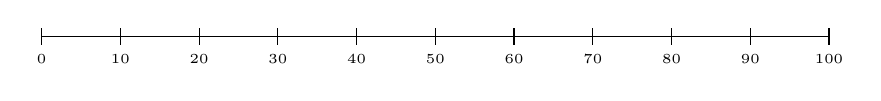
\begin{tikzpicture}[scale=1]
	\draw[-] (0,0) -- (10,0) ;
	\foreach \x in  {0,1,2,3,4,5,6,7,8,9,10}
	\draw[shift={(\x,0)},color=black] (0pt,3pt) -- (0pt,-3pt);
	\foreach \x in {0,1,2,3,4,5,6,7,8,9,10}
		\pgfmathtruncatemacro{\Result}{\x*10}
		\draw[shift={(\x,0)},color=black] (0pt,0pt) -- (0pt,-3pt) node[below] {\tiny \Result};
	\end{tikzpicture}
	\end{center}
	
\end{frame}


\frame{
	\frametitle{{\normalsize Example: Agree/Disagree (bipolar)}}

	\small
	To what extent do you agree with the following statement: I support Great Britain's participation in U.S.-led air strikes on Islamic State (IS) in Iraq and Syria.
	\begin{itemize}
		\item Strongly agree
		\item Somewhat agree
		\item Neither agree nor disagree
		\item Somewhat disagree
		\item Strongly disagree
	\end{itemize}
}

\frame{
	\frametitle{{\normalsize Example: Agree/Disagree (unipolar)}}
	
	\small
	
	To what extent do you agree with the following statement: I support Great Britain's participation in U.S.-led air strikes on Islamic State (IS) in Iraq and Syria.
	\begin{itemize}
		\item Agree completely
		\item Agree to a large extent
		\item Agree to a moderate extent
		\item Agree a little bit
		\item Agree not at all
	\end{itemize}
}

\frame{
	\frametitle{{\large Example: Forced choice}}
	When thinking about Great Britain's participation in U.S.-led air strikes on Islamic State (IS) in Iraq and Syria, which of the following comes closer to your opinion:
	\begin{itemize}
		\item Great Britain should participate in air strikes
		\item Great Britain should not participate in air strikes
	\end{itemize}
}

\frame{
	\frametitle{{\large Example: Open-ended}}
	In your own words, how would you describe your opinion on Great Britain's participation in U.S.-led air strikes on Islamic State (IS) in Iraq and Syria?
}




\frame{}


\subsection{Sensitive Topics}
%\frame{\tableofcontents[currentsection]}

\frame{
	\frametitle{Sensitive Questions}
	\begin{itemize}\itemsep0.25em
		\item Definition: Topics ``seen as intrusive or embarrassing''
		\item<2-> Factors affecting topic sensitivity
		    \begin{itemize}
                \item<2-> Individual differences
    		    \item<2-> Mode
    		    \item<2-> Interviewer
    		    \item<2-> Survey context
    		    \item<2-> Survey sponsorship
    		    \item<2-> Perceived privacy
		    \end{itemize}
		\item<3-> Why do we care?
	\end{itemize}
}

\frame{
	\frametitle{{\large Sensitive Questions Activity}}

	\small 
	
	\begin{enumerate}\itemsep0.5em
	\item<2-> To the nearest \textsterling 1,000, what is your parents' total household income?
	\item<3-> Have you ever stolen anything from a current or former employer?
	\item<4-> When was the last time you had unprotected sex?
	\item<5-> During today's lecture, how much time have you spent on your computer on things unrelated to this course?
	\end{enumerate}
}

\frame{
	\frametitle{Eliciting Sensitive Answers}
	\begin{itemize}\itemsep0.25em
		\item Ensure privacy, anonymity, or confidentiality
		\item Change modes
		\item Indirect measures
		\item Provide population base rates
		\item Placement in survey instrument
	\end{itemize}
}

\frame{}






\section[Elites]{Elite Interviewing}
\frame{\tableofcontents[currentsection]}

\frame{
\frametitle{Elite Interviewing}
\begin{itemize}\itemsep1em
\item Rules of questionnaire design style apply
\item Unique challenges/opportunities:
	\begin{itemize}
	\item Time constraints
	\item Guarantees of anonymity?
	\item Public information may be available
	\item Often exempt from research ethics review
	\end{itemize}
\end{itemize}
}

\frame{
	\frametitle{{\large Structured versus Unstructured}}
	\begin{itemize}\itemsep0.75em
	\item ``Structured'' interviews
		\begin{itemize}
		\item Strict order of questions
		\item Questions are precisely worded
		\item Often, closed set of response categories
		\end{itemize}
	\item<2-> Elite interviews often ``semi-structured''
		\begin{itemize}
		\item Greater use of open-ended questions
		\item More flexible ordering of questions
		\item More respondent-driven
		\end{itemize}
	\end{itemize}
}





\appendix
\frame{}

\end{document}
